\documentclass{article}

% This is a custom command that stretches the vertical spacing between lines
% so they're a little easier to read for this presentation
\renewcommand{\baselinestretch}{1.5} 

% For this document, we'll need some functionality not built in to LaTex, so we'll import a package.
% Here, we use hyperref to get commands that allow clickable URLs to be embedded in the PDF.
\usepackage{hyperref}
\usepackage{amsmath}
\usepackage{graphicx}

% Just like before, we'll set a few variables for the title page
\author{D. Zack Garza}
\title{A Slightly More Advanced \LaTeX Document}
\date{\today} 
% You could also just leave the date blank.


\begin{document}

% Now we'll add a title and a TOC, and put them on their own pages.
% Note that sometimes, you may need to compile your document twice for Latex to 
% get all of the TOC names and page numbers correct
\maketitle
\newpage
\tableofcontents
\newpage


% Now we'll start in on the main content

% This command is available in the document classes article and report.
\begin{abstract}
    Most research papers have this section; it's also useful for reports.
\end{abstract}


\section{Modes}
    There are two modes when typing in \LaTeX - text mode (which is what this sentence is in), and math mode.
    
    Text mode takes most characters literally, so things like x^2 don't quite work.
    
    Entering math mode can be done by enclosing text in \$ or \$\$, as seen earlier, or by using a special "environment", which we'll see shortly. Then things like $x^2$ work a bit better.
    
    But don't mix your modes! $Typing text in math mode doesn't turn out well.$ (Not by default anyways)


\section{Symbols}
    Certain characters are reserved for the underlying Tex language. To produce them, you just need to escape them with a backslash.

    \textbackslash (backslash) is used to escape characters
    
    \textbackslash\textbackslash (double backslash) is used to manually entire a line break
    
    \textasciitilde (tilde) is used to insert spacing between characters
    
    \# (number sign) is used for parameters to macros
    
    \$ (USD) is used to begin and end math mode
    
    \% (percent) is used to denote a comment
    
    \& (ampersand) is used to align things
    
    \_ (underscore) is used for subscripts 
    
    \{ and \} are generally used for grouping things


\section{Text Formatting}
    You can do the standard sort of formatting you'd expect from any word editor:
    
    \textbackslash textbf{} is used to make words \textbf{bold}.
    
    \textbackslash textit{} is used to make words \textit{italic}.
    
    \textbackslash underline{} is used to \underline{underline} words.


\section{Environments}
    Before seeing all of the math syntax we'll need, we have to take a brief interlude to discuss environments. Environments are commands that come in pairs, with a "begin" command that needs to be match to an "end" command.
    
    We've already seen one example - the document environment, which is where all of our content goes. You can use other environments in the same way; here are a few commonly used examples:

    \subsection{center}
        \begin{center}
            The \textbf{center} environment centers whatever's in it.
        \end{center}
        
        \subsection{tabular}
        The \textbf{tabular} environment lets you align things in a table:
        \begin{tabular}{ c c c } 
          cell1 & cell2 & cell3 \\ 
          cell4 & cell5 & cell6 \\ 
          cell7 & cell8 & cell9 \\ 
        \end{tabular}

        Notes: here, \textbackslash\textbackslash is used to tell the environment where each row ends.
        
        The tabular environment takes mandatory options to specify how many columns there are, and how they should be aligned.
        
        Here, the three 'c's denote 3 \textbf{center-aligned} columns. 
        
        You could also choose 'l' for \textbf{left-aligned} or 'r' for \textbf{right-aligned} columns.
        
        Note that the number of letters in the argument must match the number of columns!
        
        The \& symbol then functions as the "anchor points" for how the alignment is performed. The point where the 1st \& occurs on each row will all be aligned in a vertical column, and the 2nd and 3rd are all grouped similarly.

    \subsection{center + tabular}
        You can also combine these two environments:
        
        \begin{center}
            \begin{tabular}{| l | l | l | p{5cm} |}
            \hline
            Day & Min Temp & Max Temp & Summary \\ \hline
            Monday & 11C & 22C & A clear day with lots of sunshine.
            However, the strong breeze will bring down the temperatures. \\ \hline
            Tuesday & 9C & 19C & Cloudy with rain, across many northern regions. Clear spells 
            across most of Scotland and Northern Ireland, 
            but rain reaching the far northwest. \\ \hline
            Wednesday & 10C & 21C & Rain will still linger for the morning. 
            Conditions will improve by early afternoon and continue 
            throughout the evening. \\
            \hline
            \end{tabular}
        \end{center}
        
        Here we just added a few more things: the \textbar~ symbol places vertical bars between each column.
        
        The "p\{5cm\}" in the last column is another option that styles the contents like a paragraph of text, and allows setting a manual width so the table doesn't overflow the side of the page.
        
        The \textbackslash hline command creates horizontal lines. \\\\
        
        \textbf{A Note on Tables:} The table functionality built into \LaTeX is very powerful, but also very tricky to get right. It's often easier to design your table layout in an external editor first, then copy-paste the code into your document.
        
        One such editor that I recommend is \url{http://www.tablesgenerator.com/}

    \subsection{enumerate}
        Enumerate is used to make \textbf{ordered} lists, and will automatically number the elements.
        
        \begin{enumerate}
          \item First Item
          \item Another Item
          \item Even more items
          
          You can also just add text, it'll align to the last "item" command.
        \end{enumerate}
    
    \subsection{itemize}
        Itemize is used for \textbf{unordered} lists, and will supply bulletsfor each item.
        
        \begin{itemize}
          \item An Item
          \item An Equally Good item
          
            You can still add aligned text to any item.
        
          \item Also a Good Item
          
        \end{itemize}

    \subsection{equation}
        We saw block-level equations in the last document, but there are several environments that are particularly suited to these - especially if they span multiple lines.
        \begin{equation}
            % Everything in here is automatically in math mode.
            a^2 + b^2 = c^2
            \label{eq:pythagoras} % Here we make up a "shortcut" that we'll refer back to lter
        \end{equation}
        
        Why is this better than using \$\$?
        
        Notice the (1) that was added on the right hand side automatically - the equation environment will automatically number your equations, and even let you refer back to individual equations using label names. 
        
        These work automatically using the \textbackslash ref command, i.e. "See Equation (\ref{eq:pythagoras})"

        \newpage

        You can also suppress the automatic numbering using \* in the environment name:
        
        \begin{equation*}
            % Everything in here is automatically in math mode.
            a^2 + b^2 = c^2
            \label{eq:pythagoras2}
        \end{equation*}
        
        This is also useful for easily grouping together a result or calculation and, for example, boxing it:
        
        \begin{equation}
         \boxed{x = \pm \sqrt{z^2 - y^2}}
        \end{equation}
        
        However, this environment isn't the best for multi-line equations. For those, you'll want to import the AMSMath package, which provides:

    \subsection{align}
        This functions almost exactly like \textbf{equation} by default, but supports multiple lines.
        \begin{align}
         f(x) &= (x+a)(x+b) \\
              &= x^2 + (a+b)x + ab
        \end{align}
        
        You can still suppress numbering altogether with \*:
        
        \begin{align*}
         f(x) &= (x+a)(x+b) \\
              &= x^2 + (a+b)x + ab
        \end{align*}
        
        Or prevent numbering on individual lines:
        
        \begin{align}
         f(x) &= (x+a)(x+b) \nonumber \\
              &= x^2 + (a+b)x + ab
        \end{align}

    \subsection{figure}
        The figure environment is what you'll use just about any time you want to include an external image. It allows you to supply captions, and automatically handles numbering. Note that if your images are larger than the page, they will overflow! So it's a good habit to always supply the desired width.
        
        \begin{figure}
          \caption{Noncontractible paths on a torus.}
            % This does the magic of actually including the image
            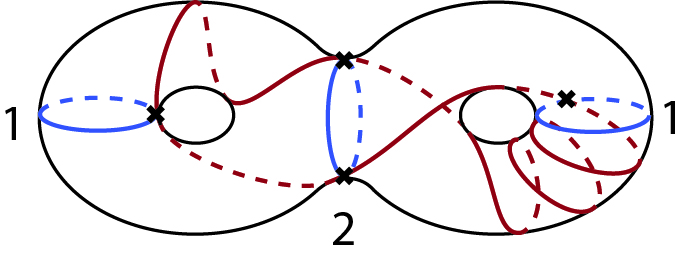
\includegraphics[width=\textwidth]{ending-3} 
        \end{figure}
        
        Note that the image doesn't always go exactly where you wrote it in the document - behind the scenes, Latex makes some default decisions about where images should be placed to keep the text flowing smoothly.
        
        You can control the placement and sizing a bit:
        \begin{figure}[h] % h denotes "here"
        \centering
          \caption{Noncontractible paths on a torus.}
            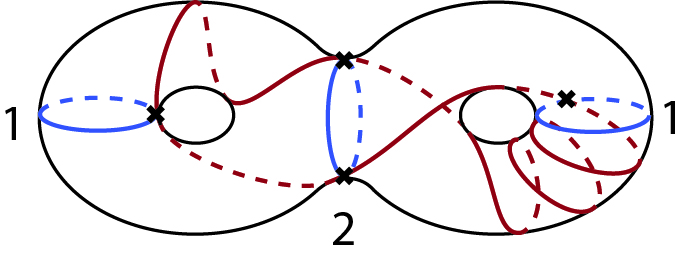
\includegraphics[width=0.5\textwidth,keepaspectratio]{ending-3}
        \end{figure}


\section{Etc}

    \subsection{Footnotes}
        You can create a footnote at any time using the \textbackslash footnote command, and it will be placed roughly on the same page as the other text surrounding it. The command will insert a hyperlink wherever you place it, though, with the number automatically assigned.\footnote{\label{myFootnoteName}I'm all the way down here!}
        
        You can also give it a label name (much like for equations), and refer to it later: "See footnote~\ref{myFootnoteName}"

    \newpage

    \subsection{Bibliography}
    Once you have the bibliography defined, you can reference it with the cite command. For example, see \cite{sourceName2} for more information.

% Most often, you would want to have a references section in your document.
% The easiest way to set this up would be by using the bibliography section
\begin{thebibliography}{1}
    % Similar to other lists, the \bibitem command can be used to list items
    % each entry can then be cited directly in the body of the text
    \bibitem{sourceName1} Amazing Source 1: www.source1.com
    \bibitem{sourceName2} Amazing Source 2: www.source2.com
\end{thebibliography}

\end{document}